\documentclass[lesson_slides]{subfiles}
%\usepackage{natbib}
\usepackage{graphicx}
% \graphicspath{ {./images/} }
\usepackage{enumerate}
\usepackage{pifont} % for ding
\usepackage{float} % keeps tables in the exact position they occupy in the code
\usepackage{xcolor} % text colour
\usepackage{gb4e} % leave last

\begin{document}
%%=-=-=-=-=-=-=-=-=-=-=-=-=-=-=-=-=-=-=-=-=-=-=-=-=-=-=-=-=-=-=-=-=-=-=-=-=-=-=-=
%   FRAME START   -=-=-=-=-=-=-=-=-=-=-=-=-=-=-=-=-=-=-=-=-=-=-=-=-=-=-=-=-=-=-=
\begin{frame}[c]{Activation of FocusP in French wh-questions}

    \transboxin<1>
    \transglitter<2>
    %\transwipe<3>
    In an earlier section, we saw that the parametrisation of FocusP can change crosslinguistically. \pause

    %\noindent \textbf{\textsc{variations in the activation of focusp}} 
    \begin{table}[H]
    \centering
        \begin{tabular}{|l|r|r|r|r|r|r|}
        \hline
         & Merge & Spell Out & Search & IM & Search\textsubscript{lex} & IM\textsubscript{lex} \\
        \hline
        Italian & 1 & 0 & 1 & 1 & 0 & 0 \\
        \hline
        Gungbe & 1 & 1 & 1 & 1 & 0 & 0 \\
        \hline
        German & 1 & 0 & 1 & 1 & 1 & 1 \\
        \hline
        \end{tabular}
    \caption{\label{tab:samp}Language variability in activating FocusP (\cite{samo2019cartography}: 147 (10)).}
    \end{table}

\end{frame}
%   FRAME END   --==-=-=-=-=-=-=-=-=-=-=-=-=-=-=-=-=-=-=-=-=-=-=-=-=-=-=-=-=-=-=
%   FRAME START   -=-=-=-=-=-=-=-=-=-=-=-=-=-=-=-=-=-=-=-=-=-=-=-=-=-=-=-=-=-=-=
\begin{frame}[c]{Activation of FocusP in French wh-questions}

\begin{center}
    \bf{The parametrisation can change even language-internally!}
\end{center}

\end{frame}
%   FRAME END   --==-=-=-=-=-=-=-=-=-=-=-=-=-=-=-=-=-=-=-=-=-=-=-=-=-=-=-=-=-=-=
%   FRAME START   -=-=-=-=-=-=-=-=-=-=-=-=-=-=-=-=-=-=-=-=-=-=-=-=-=-=-=-=-=-=-=
\begin{frame}[c]{Activation of FocusP in French wh-questions}

    \transboxin<1>
    \transglitter<2>
    \transwipe<3>
    In French, we observe four possible configurations: \pause (question-formation strategies) \pause
    \begin{itemize}
        \item[\ding{227}] \textbf{Configuration 1}: \pause in situ \pause ('T'as vu qui?')\\ \pause
        $\longrightarrow$ \pause {\bf{no wh-movement \& no verb movement}} \pause
         %%%%%%%%%%%%%%%%%% 
    \vspace*{2mm}
    \begin{table}[H]
    \centering
        \begin{tabular}{|l|r|r|r|r|}
        \hline
         & Merge & Spell Out & IM & IM\textsubscript{lex} \\
        \hline
        In situ & 1 & 0 & 0 & 0 \\
        \hline
        \end{tabular}
    \caption{\label{tab:samp}FocusP in French: Parametrisation 1.}
    \end{table}
        %%%%%%%%%%%%%%%%%%
    \end{itemize}

\end{frame}
%   FRAME END   --==-=-=-=-=-=-=-=-=-=-=-=-=-=-=-=-=-=-=-=-=-=-=-=-=-=-=-=-=-=-=
%   FRAME START   -=-=-=-=-=-=-=-=-=-=-=-=-=-=-=-=-=-=-=-=-=-=-=-=-=-=-=-=-=-=-=
\begin{frame}[c]{Activation of FocusP in French wh-questions}

    \transboxin<1>
    \transglitter<2>
    % \transwipe<3>
    In French, we observe four possible configurations: (question-formation strategies)
    \begin{itemize}
        \item[\ding{227}] \textbf{Configuration 2}: \pause SV ex situ: \pause ('Qui t'as vu?')\\ \pause
        $\longrightarrow$ \pause {\bf{wh-movement \& no verb movement}} \pause
         %%%%%%%%%%%%%%%%%% 
    \vspace*{2mm}
    \begin{table}[H]
    \centering
        \begin{tabular}{|l|r|r|r|r|}
        \hline
         & Merge & Spell Out & IM & IM\textsubscript{lex} \\
        \hline
        Ex situ & 1 & 0 & 1 & 0 \\
        \hline
        \end{tabular}
    \caption{\label{tab:samp}FocusP in French: Parametrisation 1.}
    \end{table}
        %%%%%%%%%%%%%%%%%%
    \end{itemize}

\end{frame}
%   FRAME END   --==-=-=-=-=-=-=-=-=-=-=-=-=-=-=-=-=-=-=-=-=-=-=-=-=-=-=-=-=-=-=
\begin{frame}{Activation of FocusP in French wh-questions}

    \transboxin<1>
    \transglitter<2>
    %\transwipe<3>
    \noindent \textbf{\textsc{difference between in situ and sv ex situ}} \pause
         %%%%%%%%%%%%%%%%%% 
    \vspace*{2mm}
    \begin{table}[H]
    \centering
        \begin{tabular}{|l|r|r|r|r|}
        \hline
         & Merge & Spell Out & IM & IM\textsubscript{lex} \\
         \hline
        In situ & 1 & 0 & 0 & 0 \\
        \hline
        Ex situ & 1 & 0 & 1 & 0 \\
        \hline
        \end{tabular}
    \caption{\label{tab:samp}FocusP in French: Parametrisation 2.}
    \end{table}
        %%%%%%%%%%%%%%%%%%
    
    
\end{frame}
\begin{frame}{Activation of FocusP in French wh-questions}

    \noindent \textbf{\textsc{difference between in situ and sv ex situ}}
         %%%%%%%%%%%%%%%%%% 
    \vspace*{2mm}
    \begin{table}[H]
    \centering
        \begin{tabular}{|l|r|r|r|r|}
        \hline
         & Merge & Spell Out & IM & IM\textsubscript{lex} \\
         \hline
        In situ & 1 & 0 & \hl{0} & 0 \\
        \hline
        Ex situ & 1 & 0 & 1 & 0 \\
        \hline
        \end{tabular}
    \caption{\label{tab:samp}FocusP in French: Parametrisations 1 \& 2.}
    \end{table}
        %%%%%%%%%%%%%%%%%%
    
    
\end{frame}
\begin{frame}{Activation of FocusP in French wh-questions}

    \noindent \textbf{\textsc{difference between in situ and sv ex situ}}
         %%%%%%%%%%%%%%%%%% 
    \vspace*{2mm}
    \begin{table}[H]
    \centering
        \begin{tabular}{|l|r|r|r|r|}
        \hline
         & Merge & Spell Out & IM & IM\textsubscript{lex} \\
         \hline
        In situ & 1 & 0 & 0 & 0 \\
        \hline
        Ex situ & 1 & 0 & \hl{1} & 0 \\
        \hline
        \end{tabular}
    \caption{\label{tab:samp}FocusP in French: Parametrisations 1 \& 2.}
    \end{table}
        %%%%%%%%%%%%%%%%%%
    
    
\end{frame}
%   FRAME START   -=-=-=-=-=-=-=-=-=-=-=-=-=-=-=-=-=-=-=-=-=-=-=-=-=-=-=-=-=-=-=
%   FRAME START   -=-=-=-=-=-=-=-=-=-=-=-=-=-=-=-=-=-=-=-=-=-=-=-=-=-=-=-=-=-=-=
\begin{frame}[c]{Activation of FocusP in French wh-questions}

    \transboxin<1>
    \transglitter<2>
    % \transwipe<3>
    In French, we observe four possible configurations: (question-formation strategies)
    \begin{itemize}
        \item[\ding{227}] \textbf{Configuration 3}: \pause est-ce que ex situ: \pause ('Qui est-ce que tu as vu?')\\ \pause
        Two possible interpretations:\\ \pause
        \begin{enumerate}
            \item est-ce que is a cleft with inversion \pause (est-ce moves to the LP)\\ \pause
        $\longrightarrow$ \pause {\bf{wh-movement \& no verb movement}} \pause
         %%%%%%%%%%%%%%%%%% 
    \vspace*{2mm}
    \begin{table}[H]
    \centering
        \begin{tabular}{|l|r|r|r|r|}
        \hline
         & Merge & Spell Out & IM & IM\textsubscript{lex} \\
        \hline
        Ex situ & 1 & 0 & 1 & 1 \\
        \hline
        \end{tabular}
    \caption{\label{tab:samp}FocusP in French: Parametrisation 3.}
    \end{table}
        %%%%%%%%%%%%%%%%%%

    \item est-ce que is an interrogative morpheme (/esk/):
        \pause (like Gungbe 'we')\\ \pause
        $\longrightarrow$ \pause {\bf{wh-movement \& head activation}} \pause
         %%%%%%%%%%%%%%%%%% 
    \vspace*{2mm}
    \begin{table}[H]
    \centering
        \begin{tabular}{|l|r|r|r|r|}
        \hline
         & Merge & Spell Out & IM & IM\textsubscript{lex} \\
        \hline
        Ex situ & 1 & 1 & 1 & 0 \\
        \hline
        \end{tabular}
    \caption{\label{tab:samp}FocusP in French: Parametrisation 4.}
    \end{table}
    \end{enumerate}
    \end{itemize}

\end{frame}
%   FRAME END   --==-=-=-=-=-=-=-=-=-=-=-=-=-=-=-=-=-=-=-=-=-=-=-=-=-=-=-=-=-=-=
\begin{frame}[c]{Activation of FocusP in French wh-questions}

    \transboxin<1>
    \transglitter<2>
    % \transwipe<3>
    In French, we observe four possible configurations: (question-formation strategies)
    \begin{itemize}
        \item[\ding{227}] \textbf{Configuration 4}: \pause VS ex situ: \pause ('Qui as-tu vu?')\\ \pause
        $\longrightarrow$ \pause {\bf{wh-movement \& head activation \& verb movement}} \pause
         %%%%%%%%%%%%%%%%%% 
    \vspace*{2mm}
    \begin{table}[H]
    \centering
        \begin{tabular}{|l|r|r|r|r|}
        \hline
         & Merge & Spell Out & IM & IM\textsubscript{lex} \\
        \hline
        Ex situ & 1 & 1 & 1 & 1 \\
        \hline
        \end{tabular}
    \caption{\label{tab:samp}FocusP in French: Parametrisation 1.}
    \end{table} \pause
        %%%%%%%%%%%%%%%%%%

    \noindent Why head activation?\\ \pause
    French enclitics are phi-features of C (Roberts 2007 and references therein).
    \end{itemize}

\end{frame}
%   FRAME END   --==-=-=-=-=-=-=-=-=-=-=-=-=-=-=-=-=-=-=-=-=-=-=-=-=-=-=-=-=-=-=
\begin{frame}{Activation of FocusP in French wh-questions}

    \transboxin<1>
    \transglitter<2>
    %\transwipe<3>
    \noindent \textbf{\textsc{difference between the three types of ex situ}} \pause
         %%%%%%%%%%%%%%%%%% 
    \vspace*{2mm}
    \begin{table}[H]
    \centering
        \begin{tabular}{|l|r|r|r|r|}
        \hline
         & Merge & Spell Out & IM & IM\textsubscript{lex} \\
         \hline
        Ex situ SV & 1 & 0 & 1 & 0 \\
        \hline
        Ex situ est-ce que 1 (est-ce moves) & 1 & 0 & 1 & 1 \\
        \hline
        Ex situ est-ce que 2 (/esk/) & 1 & 1 & 1 & 0 \\
        \hline
        Ex situ VS & 1 & 1 & 1 & 1 \\
        \hline
        \end{tabular}
    \caption{\label{tab:samp}FocusP in French: Ex situ parametrisations.}
    \end{table}
        %%%%%%%%%%%%%%%%%%
    
    
\end{frame}
%   FRAME END   --==-=-=-=-=-=-=-=-=-=-=-=-=-=-=-=-=-=-=-=-=-=-=-=-=-=-=-=-=-=-=
\begin{frame}{Activation of FocusP in French wh-questions}

    \noindent \textbf{\textsc{difference between the three types of ex situ}}
         %%%%%%%%%%%%%%%%%% 
    \vspace*{2mm}
    \begin{table}[H]
    \centering
        \begin{tabular}{|l|r|r|r|r|}
        \hline
         & Merge & Spell Out & IM & IM\textsubscript{lex} \\
         \hline
        Ex situ SV & \hl{1} & 0 & 1 & 0 \\
        \hline
        Ex situ est-ce que 1 (est-ce moves) & \hl{1} & 0 & 1 & 1 \\
        \hline
        Ex situ est-ce que 2 (/esk/) & \hl{1} & 1 & 1 & 0 \\
        \hline
        Ex situ VS & \hl{1} & 1 & 1 & 1 \\
        \hline
        \end{tabular}
    \caption{\label{tab:samp}FocusP in French: Ex situ parametrisations.}
    \end{table}
        %%%%%%%%%%%%%%%%%%
    
    
\end{frame}
%   FRAME END   --==-=-=-=-=-=-=-=-=-=-=-=-=-=-=-=-=-=-=-=-=-=-=-=-=-=-=-=-=-=-=
\begin{frame}{Activation of FocusP in French wh-questions}

    \noindent \textbf{\textsc{difference between the three types of ex situ}}
         %%%%%%%%%%%%%%%%%% 
    \vspace*{2mm}
    \begin{table}[H]
    \centering
        \begin{tabular}{|l|r|r|r|r|}
        \hline
         & Merge & Spell Out & IM & IM\textsubscript{lex} \\
         \hline
        Ex situ SV & \hl{1} & 0 & \hl{1} & 0 \\
        \hline
        Ex situ est-ce que 1 (est-ce moves) & \hl{1} & 0 & \hl{1} & 1 \\
        \hline
        Ex situ est-ce que 2 (/esk/) & \hl{1} & 1 & \hl{1} & 0 \\
        \hline
        Ex situ VS & \hl{1} & 1 & \hl{1} & 1 \\
        \hline
        \end{tabular}
    \caption{\label{tab:samp}FocusP in French: Ex situ parametrisations.}
    \end{table}
        %%%%%%%%%%%%%%%%%%
    
    
\end{frame}
%   FRAME END   --==-=-=-=-=-=-=-=-=-=-=-=-=-=-=-=-=-=-=-=-=-=-=-=-=-=-=-=-=-=-=
\begin{frame}{Activation of FocusP in French wh-questions}

    \noindent \textbf{\textsc{difference between the three types of ex situ}}
         %%%%%%%%%%%%%%%%%% 
    \vspace*{2mm}
    \begin{table}[H]
    \centering
        \begin{tabular}{|l|r|r|r|r|}
        \hline
         & Merge & Spell Out & IM & IM\textsubscript{lex} \\
         \hline
        Ex situ SV & \hl{1} & 0 & \hl{1} & 0 \\
        \hline
        Ex situ est-ce que 1 (est-ce moves) & \hl{1} & 0 & \hl{1} & 1 \\
        \hline
        Ex situ est-ce que 2 (/esk/) & \hl{1} & \textcolor{red}{1} & \hl{1} & 0 \\
        \hline
        Ex situ VS & \hl{1} & \textcolor{red}{1} & \hl{1} & 1 \\
        \hline
        \end{tabular}
    \caption{\label{tab:samp}FocusP in French: Ex situ parametrisations.}
    \end{table}
        %%%%%%%%%%%%%%%%%%
    
    
\end{frame}
%   FRAME END   --==-=-=-=-=-=-=-=-=-=-=-=-=-=-=-=-=-=-=-=-=-=-=-=-=-=-=-=-=-=-=
\begin{frame}{Activation of FocusP in French wh-questions}

    \noindent \textbf{\textsc{difference between the three types of ex situ}}
         %%%%%%%%%%%%%%%%%% 
    \vspace*{2mm}
    \begin{table}[H]
    \centering
        \begin{tabular}{|l|r|r|r|r|}
        \hline
         & Merge & Spell Out & IM & IM\textsubscript{lex} \\
         \hline
        Ex situ SV & \hl{1} & 0 & \hl{1} & 0 \\
        \hline
        Ex situ est-ce que 1 (est-ce moves) & \hl{1} & 0 & \hl{1} & \textcolor{orange}{1} \\
        \hline
        Ex situ est-ce que 2 (/esk/) & \hl{1} & \textcolor{red}{1} & \hl{1} & 0 \\
        \hline
        Ex situ VS & \hl{1} & \textcolor{red}{1} & \hl{1} & \textcolor{orange}{1} \\
        \hline
        \end{tabular}
    \caption{\label{tab:samp}FocusP in French: Ex situ parametrisations.}
    \end{table}
        %%%%%%%%%%%%%%%%%%
    
    
\end{frame}
%   FRAME END   --==-=-=-=-=-=-=-=-=-=-=-=-=-=-=-=-=-=-=-=-=-=-=-=-=-=-=-=-=-=-=
\begin{frame}{Summing up}
    \begin{center}
        \textbf{Summing up: possible setting combinations for the French FocusP.}
    \end{center}
\end{frame}
%   FRAME START   -=-=-=-=-=-=-=-=-=-=-=-=-=-=-=-=-=-=-=-=-=-=-=-=-=-=-=-=-=-=-=
\begin{frame}[c]{Combinations for French}

    \begin{center}
        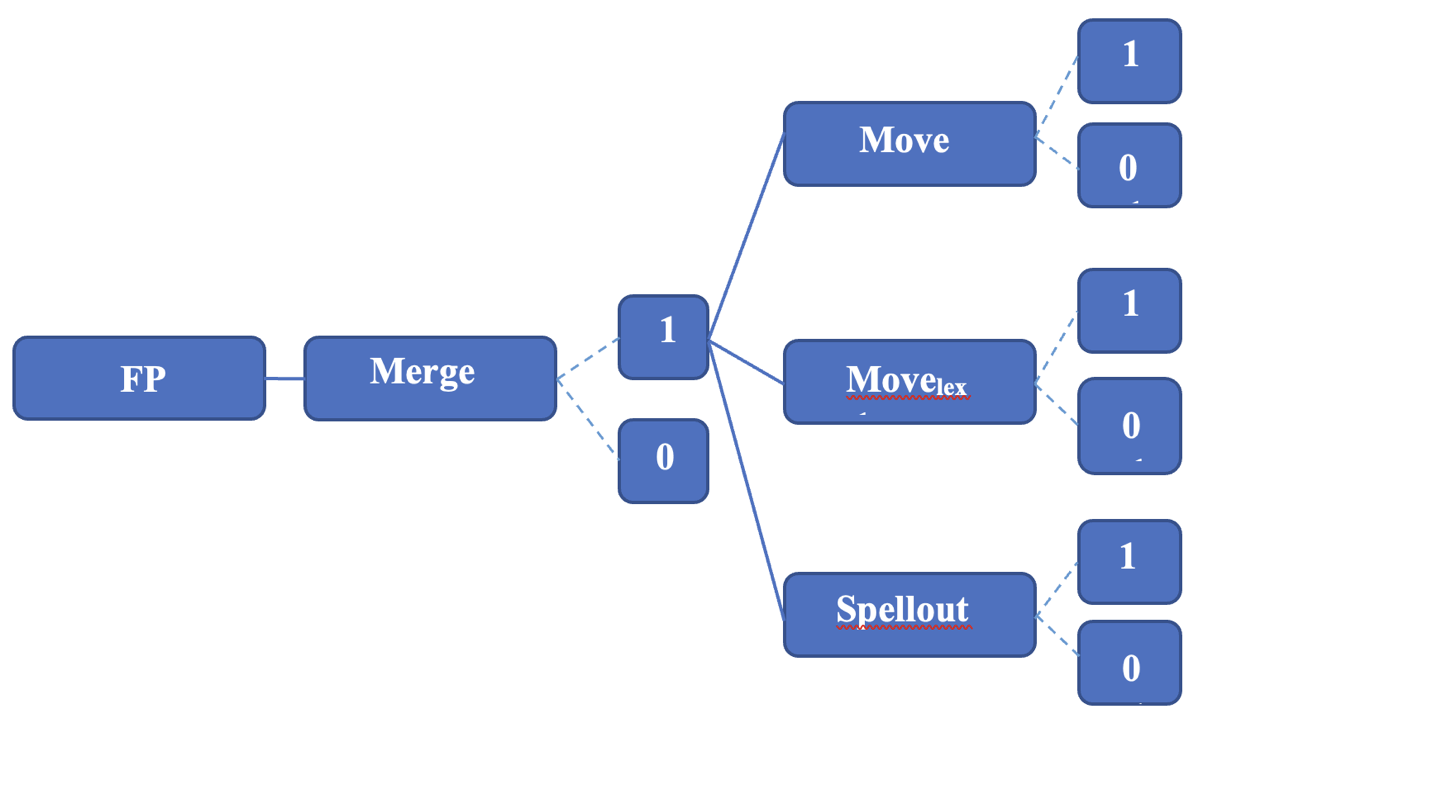
\includegraphics[width=12cm, height=6cm]{images/combinationsfrenchb.png}
    \end{center}

\end{frame}
%=-=-=-=-=-=-=-=-=-=-=-=-=-=-=-=-=-=-=-=-=-=-=-=-=-=-=-=-=-=-=-=-=-=-=-=-=-=-=-=
%   FRAME START   -=-=-=-=-=-=-=-=-=-=-=-=-=-=-=-=-=-=-=-=-=-=-=-=-=-=-=-=-=-=-=
\begin{frame}[c]{Combinations for French}

    \begin{center}
        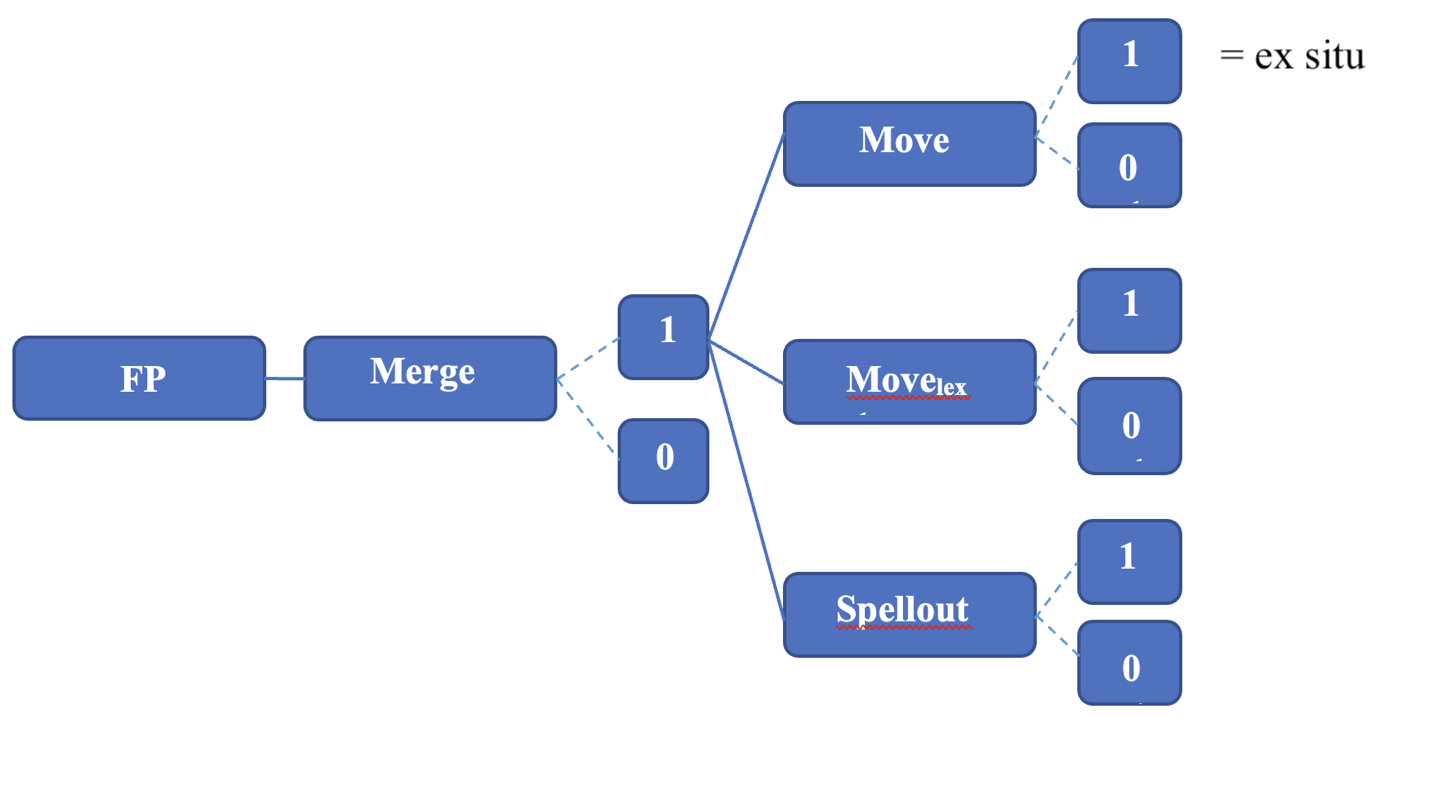
\includegraphics[width=12cm, height=6cm]{images/combinationsfrench1.png}
    \end{center}

\end{frame}
%=-=-=-=-=-=-=-=-=-=-=-=-=-=-=-=-=-=-=-=-=-=-=-=-=-=-=-=-=-=-=-=-=-=-=-=-=-=-=-=
%   FRAME START   -=-=-=-=-=-=-=-=-=-=-=-=-=-=-=-=-=-=-=-=-=-=-=-=-=-=-=-=-=-=-=
\begin{frame}[c]{Combinations for French}

    \begin{center}
        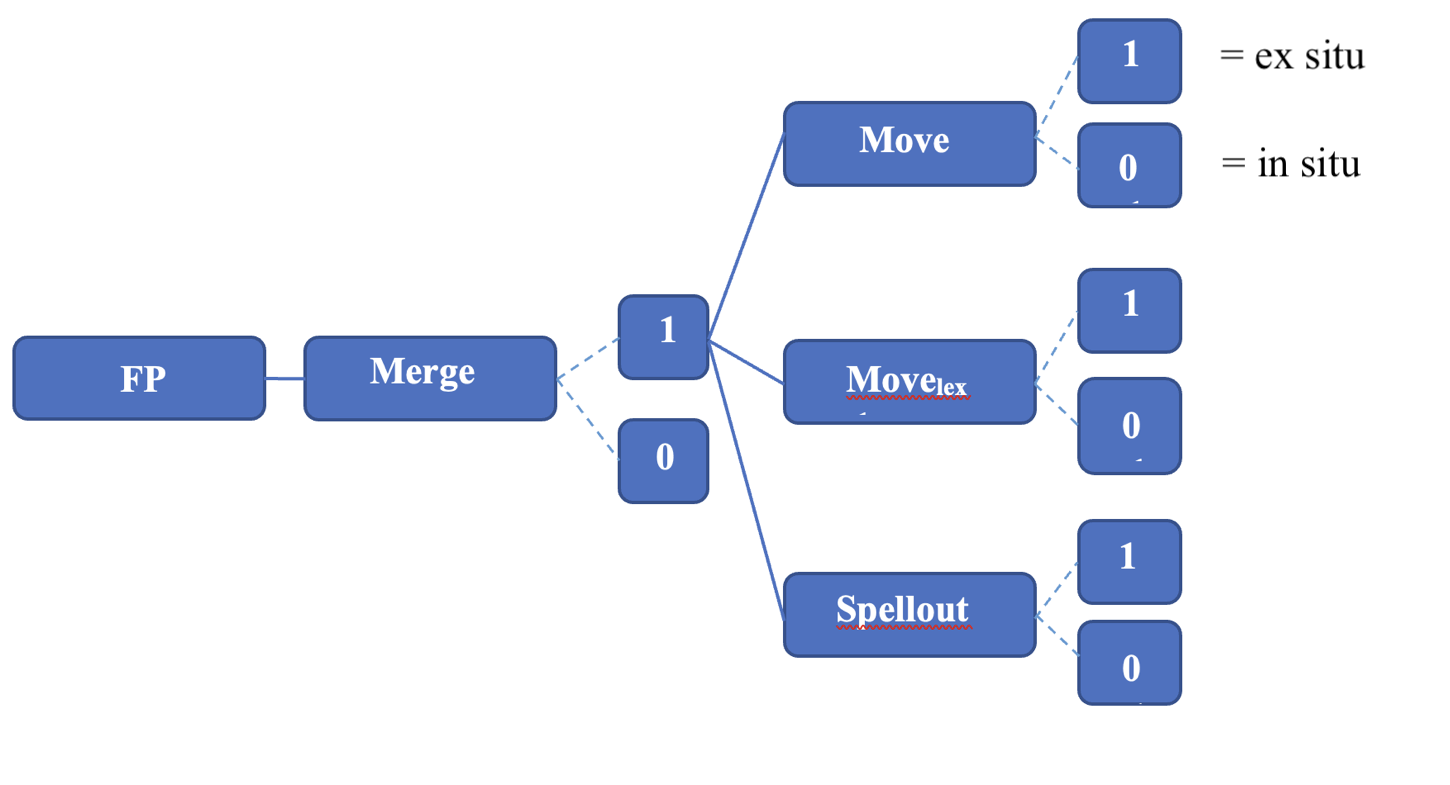
\includegraphics[width=12cm, height=6cm]{images/combinationsfrench2.png}
    \end{center}

\end{frame}
%=-=-=-=-=-=-=-=-=-=-=-=-=-=-=-=-=-=-=-=-=-=-=-=-=-=-=-=-=-=-=-=-=-=-=-=-=-=-=-=
%   FRAME START   -=-=-=-=-=-=-=-=-=-=-=-=-=-=-=-=-=-=-=-=-=-=-=-=-=-=-=-=-=-=-=
\begin{frame}[c]{Combinations for French}

    \begin{center}
        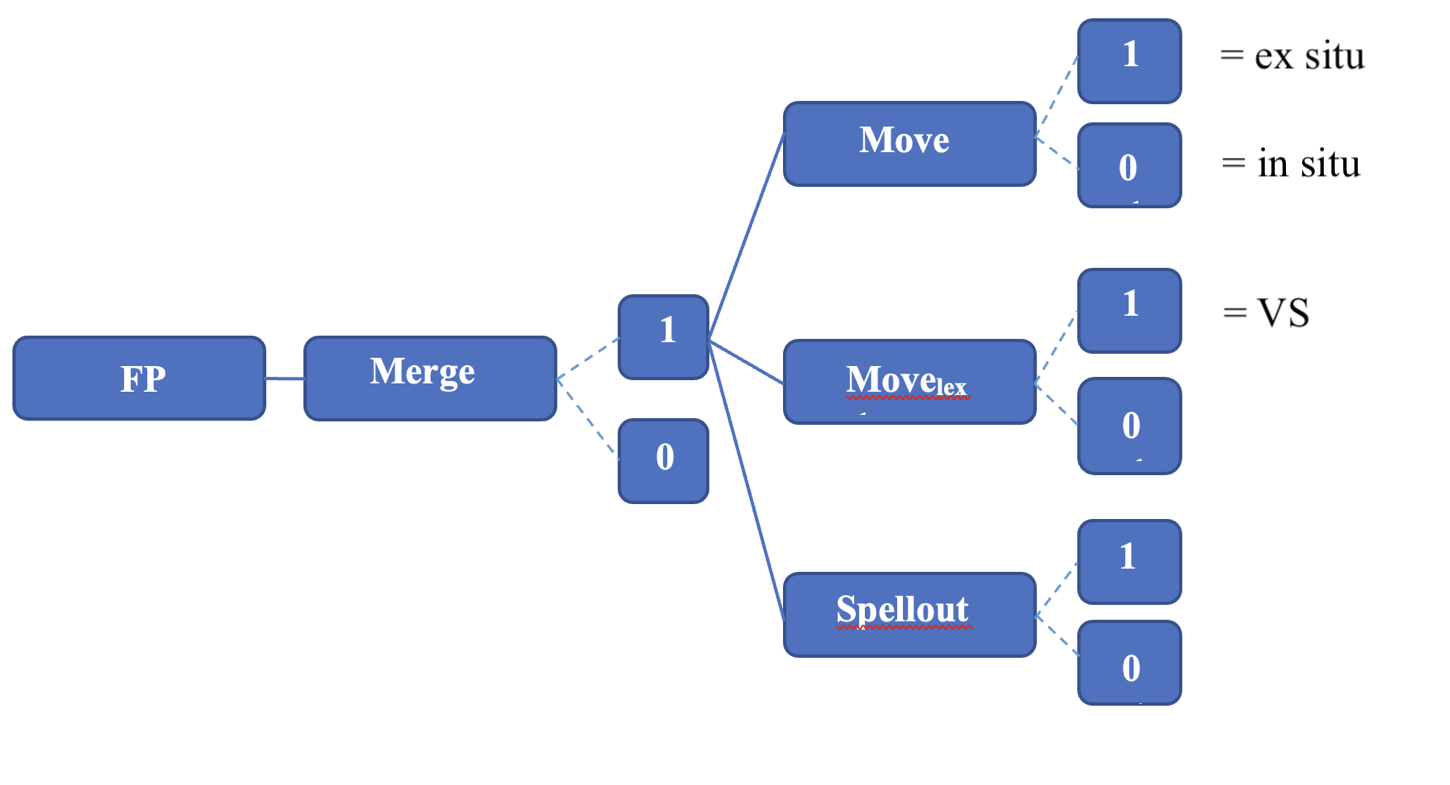
\includegraphics[width=12cm, height=6cm]{images/combinationsfrench3.png}
    \end{center}

\end{frame}
%=-=-=-=-=-=-=-=-=-=-=-=-=-=-=-=-=-=-=-=-=-=-=-=-=-=-=-=-=-=-=-=-=-=-=-=-=-=-=-=
%   FRAME START   -=-=-=-=-=-=-=-=-=-=-=-=-=-=-=-=-=-=-=-=-=-=-=-=-=-=-=-=-=-=-=
\begin{frame}[c]{Combinations for French}

    \begin{center}
        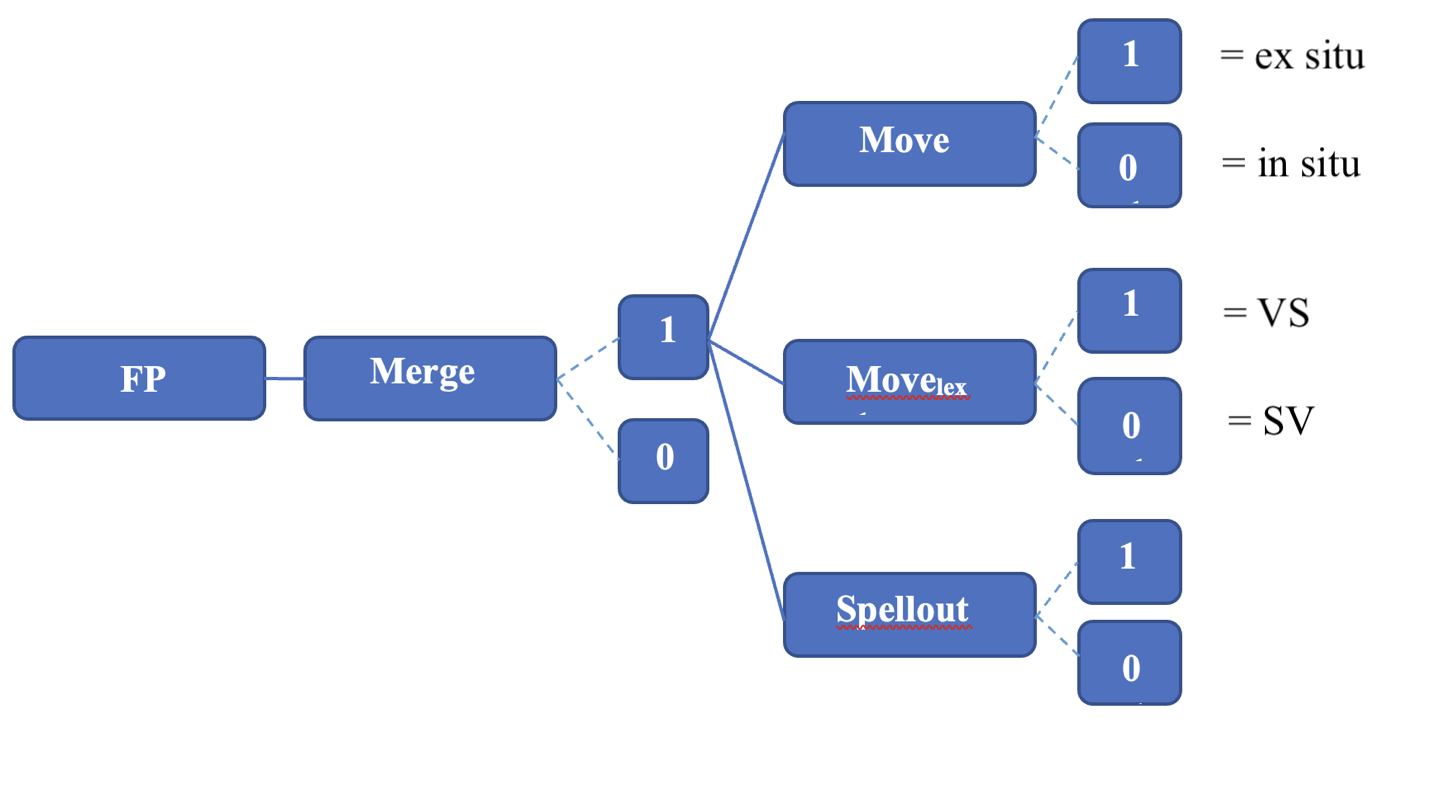
\includegraphics[width=12cm, height=6cm]{images/combinationsfrench4.png}
    \end{center}

\end{frame}
%=-=-=-=-=-=-=-=-=-=-=-=-=-=-=-=-=-=-=-=-=-=-=-=-=-=-=-=-=-=-=-=-=-=-=-=-=-=-=-=
%   FRAME START   -=-=-=-=-=-=-=-=-=-=-=-=-=-=-=-=-=-=-=-=-=-=-=-=-=-=-=-=-=-=-=
\begin{frame}[c]{Combinations for French}

    \begin{center}
        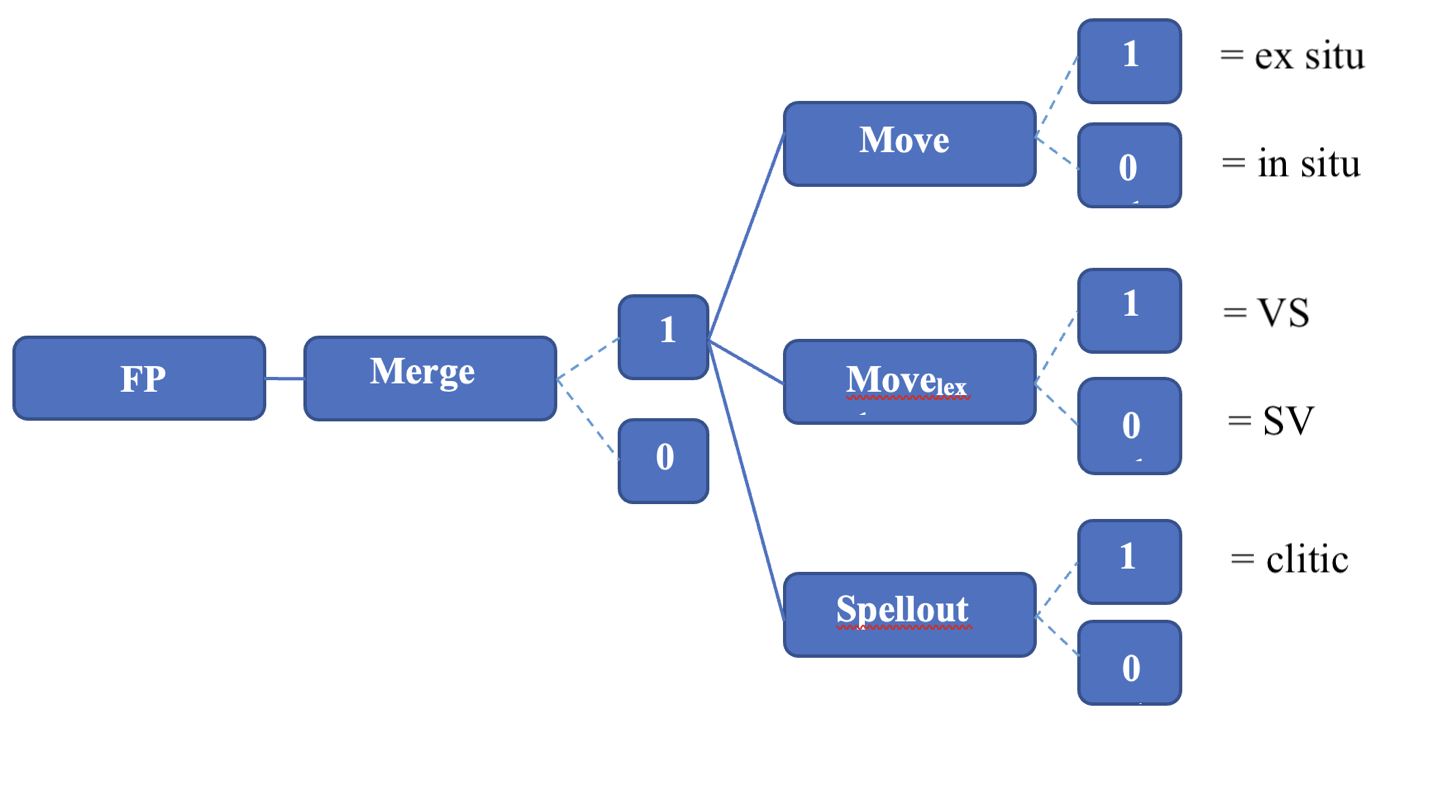
\includegraphics[width=12cm, height=6cm]{images/combinationsfrench5.png}
    \end{center}

\end{frame}
%=-=-=-=-=-=-=-=-=-=-=-=-=-=-=-=-=-=-=-=-=-=-=-=-=-=-=-=-=-=-=-=-=-=-=-=-=-=-=-=
%   FRAME START   -=-=-=-=-=-=-=-=-=-=-=-=-=-=-=-=-=-=-=-=-=-=-=-=-=-=-=-=-=-=-=
\begin{frame}[c]{Combinations for French}

    \begin{center}
        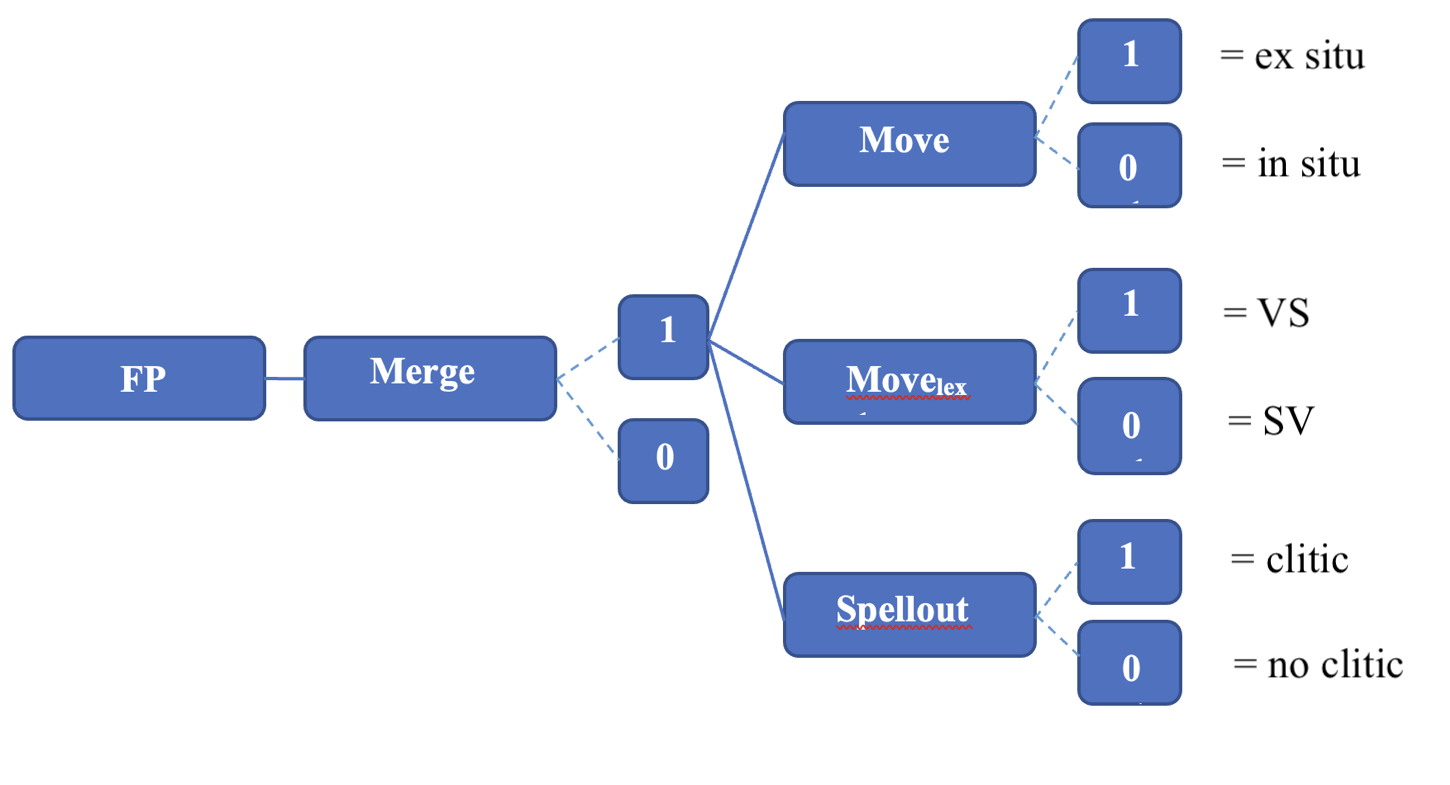
\includegraphics[width=12cm, height=6cm]{images/combinationsfrench6.png}
    \end{center}

\end{frame}
%=-=-=-=-=-=-=-=-=-=-=-=-=-=-=-=-=-=-=-=-=-=-=-=-=-=-=-=-=-=-=-=-=-=-=-=-=-=-=-=
%=-=-=-=-=-=-=-=-=-=-=-=-=-=-=-=-=-=-=-=-=-=-=-=-=-=-=-=-=-=-=-=-=-=-=-=-=-=-=-=
\end{document}